\documentclass[11pt,final]{fithesis} %aj s obrazkami
%\documentclass[11pt,draft,oneside]{fithesis} %bez obrazkov
\usepackage[plainpages=false, pdfpagelabels]{hyperref}
\usepackage[T1]{fontenc}  %aby boli pekne pismena
\usepackage[slovak]{babel}  %slovensky balik
\usepackage{longtable}     % pre vecsie tabulky
\usepackage{graphicx}
\usepackage{a4wide}
\usepackage{lettrine}  %velke uvodne pismeno

\thesistitle{Pou�itie BPMN pre mal� SW projekty}
\thesissubtitle{Diplomov� pr�ca}
\thesisstudent{Bc. Miroslav Ligas}
\thesiswoman{false}
\thesisfaculty{fi}
\thesislang{sk}
\thesisyear{jaro 2009}
\thesisadvisor{RNDr. Tom� Lud�k}

\begin{document}
\FrontMatter
\ThesisTitlePage

\begin{ThesisDeclaration}
\DeclarationText
\AdvisorName
\end{ThesisDeclaration}

\begin{ThesisThanks}
Na tomto mieste by som sa chcel r�d po�akova� ved�cemu mojej diplomovej pr�ce p�novi RNDr. Tom�ovi Lud�kovi, za jeho podporu a smerovanie pri p�san� tejto pr�ce.
\end{ThesisThanks}
\begin{ThesisAbstract} 
TBD
\end{ThesisAbstract} 
 
\begin{ThesisKeyWords} 
Business Process Modeling Notation, Unified Modeling Language, Vodop�d, Iterat�vny / inkrement�lny v�voj, Agiln� met�dy v�voja, Business Driven Development, Servisne Orientovan� Architekt�ru
\end{ThesisKeyWords} 
 
\MainMatter
\tableofcontents
\chapter{�vod}
\label{chap:uvod}
S rie�en�m softv�rov�ch projektov vznikaj� r�zne probl�my, ktor� m��u vies� k zlyhaniu projektu. Tieto rizik� sa pri v�voji sna��me odstr�ni� zaveden�m metod�k, ktor� n�m napom�haj� uchopi� projekt, rozanalyzova� problematick� miesta a �o najlep�ie navrhn�� rie�enie. �iadna metodika n�m nezaist� splnite�nos� projektu ale jej pou�itie minimalizuje riziko krachu projektu. 

Najpou��vanej�ie modelovacie metodiky s��asnej doby s� ve�mi rozsiahle a siln� n�stroje. Definuj� ve�k� mno�stvo roli a zav�dzaj� komplexn� procesy, ��m dok�u zvl�da� ve�k� projekty. Vn�aj� t�m do v�voja ve�k� r�iu, ktor� projekt pom�ha lep�ie zvl�da� ale ho aj predl�uje. ��m je projekt men�� t�m je cite�nej�ia z�a� komplexnej metodiky. Opomenutie metod�k by zbavilo projekty v�etkej r�ie a u�etrilo by �as aj prostriedky, ale riziko, ktor� by vzniklo by mnohon�sobne prev��ilo �sporu. 

Pri modernom v�voji nie je preto rozumn� postupova� bez metodik pri akomko�vek v�voji. Napriek tomu sa naskytuje priestor na h�adanie nov�ch ciest pri ich rie�en�. Namiesto vyu��vania rozsiahlych pou��van�ch a overen�ch metodik sa treba zamera� na ich esenci�lne �asti. Na z�klade t�chto �ast� sa vybuduje �ahko zvl�dnute�n� a flexibiln� met�da. 

Mal� softv�rov� projekty s� v��inou sprac�van� neve�k�m po�tom pracovn�kov ako na strane v�voj�ra tak na strane klienta. Ukazuje sa tu preto miesto pre r�chlu a flexibiln� met�du, ktor� dok�e r�chlo produkova� funk�n� moduly a flexibilne reagova� na po�iadavky klienta. Cie�om tejto pr�ce je n�js� stanoven� met�du.

\section{�trukt�ra pr�ce}

Druh� kapitola pr�ce sa zaober� najpou��vanej��mi modelovac�mi n�strojmi, ktor� sa v s��asnosti pou��vaj� na zachytenie interakcie a stavu v danom syst�me. Podrobne sa  tu popisuje roz��ren� no mo�no nie tak notoricky zn�mi n�stroj na modelovanie firemn�ch procesov Business Process Modeling Notation (BPMN). Okrajovo sa spom�na aj Unified Modeling Language (UML). Popisovan� s� len niektor� prvky UML, s ktor�mi sa v pr�ci stretneme. \\

Tretia kapitola je venovan� metodik�m. Popisuje r�zne pr�stupy ako rie�i� budovanie syst�mu. Zaober� sa agiln�mi  metodikami, ktor� sa vyzna�uj� r�chlos�ou a flexibilitou. V kontraste k nim stoja tradi�n� �trukt�rovan� metodiky ako Unified Process (UP), ktor� stavaj� na definovan�ch postupoch a roliach. Podrobnej�ie sa venujeme najm� t�m, z�ktor�ch �erp�me in�pir�ciu pre zostavenie vlastnej met�dy. \\

�tvrt� kapitola zachyt�va hlavn� �as� pr�ce a to definovanie met�dy pre mal� softv�rov� projekty s vyu�it�m BPMN. V tejto kapitole sa uplat�uj� n�stroje a postupy definovan� v predch�dzaj�cich oddieloch.  Met�da je zostaven� zo zau��van�ch metod�k, z ktor�ch sa vyberaj� relevantn� �asti. Sp�ja sa v nej agiln� pr�stup a tradi�n� �trukt�rovan� metodiky. Metoda �erp� inspir�ciu z Business Driven Development (BDD) z dielne IBM. Na zachytenie po�iadavkov a identifik�ciu modulov v projektovanom syst�m pou��va hierarchiu BPMN diagramov. Jednotlive moduly s� n�sledne modelovan� za pomoci tradi�n�ch UML diagramov. \\

Z�vere�n� piata kapitola overuje vhodnos� definovanej met�dy. Z jej vyu�it�m je vytvoren� pr�padov� �t�dia popisuj�ca spr�vu vedeck�ho �asopisu. Pomocou uveden�ch n�strojov modeluje hierarchiu procesov prebiehaj�cich pri fungovan� spr�vy vedeck�ho �asopisu. Vo vzniknutej procesnej mape s� identifikovan� procesy, ktor� je mo�n� automatizova�. N�sledne s� ur�ene komponenty, ktor� s� pomocou UML modelovan� a na z�ver je na�rtnut� implement�cia. \\
\chapter{Modelovacie n�stroje}
\label{chap:nastroje}
obkec o BPM 

\chapter{Pr�stupy k vyvoju softv�ru}
\label{chap:metodmod}
obkec okolo metodik

\section{Inkrement�lny}
\label{sec:increm}

\section{Iitera�n�}
\label{sec:spiral}

\section{Agiln� metodiky}
\label{sec:agil}

\section{Business Driven Development}
\label{sec:bdd}

\section{Unified Process}
\label{sec:up}
\chapter{N�vrh v�vojovej met�dy}
\label{chap:momet}
Cie�om tejto kapitoly jej navrhn�� met�du pre v�voj mal�ch softv�rov�ch projektov. Vyu�ijeme pri tom zozbieran� znalosti o modern�ch pr�stupoch k navrhovaniu syst�mov. Met�da bude zameran� na maxim�lnu efektivitu. V�voj postupuj�ci pod�a navrhnutej met�dy mus� zvl�dnu� t�m minim�lnej ve�kosti. Met�da bude zalo�en� na osved�en�ch a u� dlh� roky pou��van�ch metodik�ch, ktor� bud� tvori� jej z�klad a bude vych�dza� z ich pozit�vnych vlastnost�. 

Hlavnou snahou navrhovanej met�dy je minimaliz�cia prostriedkov a �silia, ktor� priamo nevedie k tvoreniu syst�mu. Met�da bude sl��i� na v�voj mal�ch projektov ktor� s� �ahko uchopite�n� pre odborn�ka a preto rozsiahle modelovanie probl�mu nie je efekt�vne. Bude tu snaha o potla�enie nepotrebnej byrokracie a nadbyto�n�ho produkovania modelov a dokument�cii. Na druhej strane nesmie by� v�ak ohrozen� spo�ahlivos� met�dy, ktor� by sa prejavila zlyhan�m projektu.

\section{Charakteristika met�dy}

Pri modelovan� novej met�dy mus�me ako prv� krok zostavi� jej charakteristiku. Pop��eme t�m z�kladn� vlastnosti, ktor� bud� met�du charakterizova� a ur�ova� ak�m sp�sobom bude fungova�. In�pir�ciu pre stanovenie z�kladn�ch ��t m��eme �erpa� z historicky star��ch metod�k. M��eme sa opiera� o v�hody a nev�hody z�skan� ich pou��van�m. Na z�klade t�chto znalosti vyberieme tak� vlastnosti, ktor� bud� pre charakter n�ho projektu najvhodnej�ie.   

\subsection{Model �ivotn�ho cyklu}

Ako prv� sa zamysl�me nad najvhodnej��m modelom pre na�u met�du. Medzi historicky najstar�ie modely patr� model vodop�d. Tomuto modelu sme sa venovali v tretej kapitole \ref{sec:vod}. Je zalo�en� na line�rnom postupe skrz f�zy v�voja. Jeho pr�nosom je jasn� definovanie �innost� v�voja a jeho postupnost�. V s��astnosti je tento postup prekonan�, lebo len �a�ko sa s n�m zvl�daj� zlo�itej�ie projekty. Hlavnou nev�hodou okrem neflexibility a zlo�itej opravy ch�b je dlh� �asov� �sek od zadania projektu do doby kedy sa z�kazn�k m��e stretn�� s objednanou aplik�ciou. Modern� n�vrh v�ak nezabudol na vodop�d, ale vyu��va jeho vylep�enia.

Jedn�m z najroz��renej��ch modelov, ktor� vych�dzaj� z vodop�du a pou��vaj� sa v modern�ch n�vrhoch je iterat�vny model. Rozde�uje probl�m na men�ie podprobl�my na z�klade funkcionality. Pre ka�d� �iasto�n� �lohu sa potom vykon�va anal�za, n�vrh, implement�cia a testovania. Prebieha tu vlastne mal� vodop�d. Pracovanie s men��mi funk�n�mi �as�ami, u�ah�uje zvl�dnutie aj zlo�itej��ch projektov. Koncov� produkt z�skame po vykonan� v�etk�ch iter�ci�. �asto sa tento pr�stup kombinuje s inkrement�lnym v�vojom, ktor�ho pr�nosom je postupn� vyv�janie syst�mu v samostatn�ch �astiach. Projekt je rozdelen� na inkrementy, ktor� sa osobitne vyv�jaj�. Inkrementy s� po ich dokon�en� integruj� do v�sledn�ho rie�enia. Podrobnej�ie boli obidva modely pop�san� v tretej kapitole \ref{sec:InIt}. \\

Z vopred z�skan�ch znalost� je ako najvhodnej�� pr�stup vybran� itera�no-inkrement�lny model. Umo��uje n�m vyv�ja� aplik�ciu postupne, ��m zni�uje riziko zlyhania projektu a taktie� umo��uje dod�va� z�kazn�kovi priebe�ne verzie syst�mu, ku ktor�m sa z�kazn�k m��e vyjadri�. Vybran� model si mierne pooprav�me pre na�e potreby. Ke�e pracujeme s mal�mi softv�rov�m projektami, nie je zapotreby vyu��va� ve�k� mno�stvo iter�ci� a inkrementov. Ur�enie po�tu jednotliv�ch v�vojov�ch oddielov bude hlavne z�visl� na funkcionalite bud�ceho syst�mu a na tom ako bude syst�m dod�van� z�kazn�kovi. 

\subsection{Agiln� prvky}
Pri s�dobom v�voji aplik�ci� sa st�va jedn�m z najd�le�itej��ch faktorov schopnos� v�voj�rov reagova� na r�chlo meniace sa prostredie a po�iadavky na vyv�jan� syst�m.  Klasick� met�dy s� v s��asnej dobre �a�ko efekt�vne vyu�ite�n�, lebo neposkytuj� rie�enia vo chv��ach, ke� s� zapotreby. Probl�mom zv��enia schopnosti prisp�sobenia sa aktu�lnym potreb�m z�kazn�ka sa zaoberala �as� pr�ce o agiln�ch met�dach v�voja \ref{sec:agil}.\\

V navrhovanej met�de sa budeme sna�i� vyu�i� vlastnosti agiln�ch met�d, aby bola zabezpe�en� �o najvy��ia flexibilita v�voja. 

Jedn�m z hlavn�ch bodov v agiln�ch postupoch je vysok� miera zainteresovania z�kazn�ka do procesu v�voja. Napriek tomu �e navrhovan� met�da sa m� zaobera� mal�mi projektami, ktor� by nemali by� ve�mi komplikovan� na pochopenie, mus� prevl�da� snaha o zapojenie z�kazn�ka do v�voja. Pri d�le�it�ch rozhodnutiach o porad� v�voja �ast� aplik�cie a pri ot�znych bodoch v�voja by z�kazn�k nikdy nemal ch�ba�. V pr�pade nez�ujmu zo strany objedn�vate�a m��e nasta� zn��enie kvality, pr�padne dodanie �plne ne�iad�ceho syst�mu.

Cie�om agiln�ch metod�k je �o najr�chlej�ie sa dosta� do f�ze programovania. Modelovacia a dokumenta�n� �innos� je a� na druhom mieste. V novej met�de je tie� snaha o u�etrenie n�kladov r�chlej��m prist�pen�m k programovaniu. Modelovanie a dokumentovanie sa v�ak nepova�uje za �innos� ktor� spoma�uje v�voj. Dobr� n�vrh je priam naopak sp�sob ako si �as pri v�voji u�etri�. Napriek tomu sa ale pre efektivitu obmedz�me na tie najpotrebnej�ie modely syst�mu, ktor�mi je jasne stanoven� funkcionalita. Drobn� implementa�n� detaily sa zbyto�ne pracne nemodeluj�, ale vych�dzaj�c z kvalifikovanosti program�tora, aby dan� probl�m vyrie�il.

Spolupr�ca a komunik�cia je v rie�ite�skom t�me maxim�lne d�le�it�. Pracovn�ci musia by� ochotn� pom�ha� si jedne druh�mu. Roz�iruj� t�m svoje znalosti, zvy�uj� priemern� kvalifikovanos� t�mu a dok�u sa sk�r vysporiada� s probl�mami. Minimalizuje sa form�lna komunik�cia, ktor� �asto sp�sobuje len zbyto�n� z�a� na v�vojov� proces a odda�uje �ud� v t�me. Z charakteru projektov, pre ktor� je met�da navrhovan� vypl�va, �e na ich zvl�dnutie nebude potreba ve�k� mno�stvo pracovn�kov. Pre tieto d�vody by nemalo by� obtia�ne splni� vy��ie spom�nan� po�iadavky na t�mov� pr�cu. V�etky tieto kroky s� veden� na vytvorenie pozit�vnej, kon�trukt�vnej atmosf�ry v rie�ite�skom t�me, ktor� motivuje pracovn�kov k pod�vaniu maxim�lneho v�konu a produkovania kvalitn�ch rie�en�.

\subsection{Vyu�itie BPMN}

BPMN sl��i ako grafick� jazyk, ktor� je �pecializovan� pre popis firemn�ch procesov. Podrobn� popis syntaxe bol podan� v druhej kapitole. \ref{sec:bpmn}. Modelovanie firemn�ch procesov bude sl��i� na objasnenie fungovania organiz�cie a presne ur�enie procesov, ktor� v nej prebiehaj�. V�aka t�mto procesom �ahko identifikujeme �asti, ktor� je mo�n� automatizova�. Identifikujeme pr�pady u�itia a namodelovan� procesy vyu�ijeme ako grafick� zn�zornenie krokov, ktor� treba pre dan� pr�pad u�itia vykona�. Touto �innos�ou z�skame sadu diagramov, ktor� zobrazuje firemn� procesy prepojen� na diagramy pr�padov u�itia.\\ 

Diagramy firemn�ch procesov s� pre z�kazn�ka ve�mi intuit�vne a podrobne popisuj� syst�m, ak�m organiz�cia pracuje alebo ak�m sa ur�it� modelovan� �innos� vykon�va. V kontraste s klasicky pou��van�m diagramom pr�padov u�itia, ktor� zachyt�vaj� len heslovite po�adovan� funkcionalitu, vid� z�kazn�k presn� postupy, s ktor�mi sa m��e �ahko stoto�ni�. Z�skavame tak siln� graficky model, v ktorom sa z�kazn�k �ahko dok�e orientova�. Nad vypracovan�mi diagramami je mo�nos� �ah�ej komunik�cie so z�kazn�kom, lebo m� presnej�iu predstavu o tom, �o sa v bud�com syst�me ocitne. M��e komentova� presnos� procesov a pr�padne spolu s v�voj�rom diskutova� o ich vylep�en�.

\subsection{In�pir�cia BDD}

Definovan� met�da �erp� ve�k� in�pir�ciu z Business Driven Development-u, ktor�mu sme sa venovali v tretej kapitole. \ref{sec:bdd} Preber� z BDD hlavn� my�lienku pribl��enia v�voja  k�potreb�m z�kazn�ka. Produkovan� syst�my maj� spl�ova� aktu�lne po�iadavky a maj� by� doru�en� �o najsk�r, aby poskytli pre klienta potrebn� konkuren�n� v�hodu. 

Nov� met�da vych�dza zo �ivotn�ho cyklu definovan�ho v BDD. Zjednodu�uje cely cyklus a upravuje jednotliv� f�zy, aby zaberali �o najmenej �asu a �silia. Zmeny ale neovplyv�uj� robustnos� rie�enia a nevn�aj� neistotu z ne�spechu projektu.  Podobne ako bol pretransformovan� �ivotn� cyklus, s� pozmenen� aj role. Ich kompetentnosti s� v niektor�ch pr�padoch roz��ren� a niektor� role s� naopak okresan� pr�padne �plne odstr�nen�.

Podstatnou inspir�ciu bola prv� f�za, ktor� sa venuje firemn�ch procesom a ich modelovaniu. Stala sa hybnou silou novo-navrhnutej met�dy. Nov� postup men� sp�sob a v�znam pou�itia modelovania firemn�ch procesov. Vyu��va ich na zachytenie po�iadavkov na syst�m a podobn� grafick� zn�zornenie procesov v organiz�cii, z ktor�ho je �ahk� ur�i� pr�pady u�itia a ich popis. Klient tak z�skava zrozumite�nej�� n�h�ad na bud�ci syst�m. \\

Novo-definovan� met�da prin�a aj  nov� �pecifik�, ktor� s� ovplyvnen� hlavne my�lienkami plyn�cimi z manifesta agiln�ho programovania. S� to hlavne my�lienky t�kaj�ce sa prace v t�me a potla�enia nadbyto�nej byrokracie. Ako bolo u� vy��ie zmienen�, pr�ca v t�me m� by� in�pirat�vna a povzbudzuj�ca k pod�vaniu �o najlep��ch v�sledkov.

\section{�ivotn� cyklus}
Pre navrhovan� met�du je definovan� �ivotn� cyklus, ktor� je zobrazen� na obr�zku \ref{fig:mypic}. Pokr�va v�voj od n�vrhu a� po nasadenie syst�mu. M� cyklick� charakter, ktor� n�m nazna�uje iterat�vno-inkrement�lne vylep�ovanie syst�mu pri v�voji. Proces v�voja za��na modelovan�m firemn�ch procesov. Po tejto f�zy nastane identifik�cia funk�n�ch �ast� na z�klade, ktorej sa projekt rozdel� na men�ie pod�asti. Jednotliv�mi �as�ami je ur�en� priorita a postupne prech�dzaj� v�vojov�mi f�zami. Ako prvou prech�dzaj� n�vrhom syst�mu. Vyprodukovan� modely sl��ia ako vstup do v�vojovej f�zy, ktor� je nasledovan� testovan�m.  Po ukon�en� testovania sa pou�ite�n� �as� syst�mu zav�dza do prev�dzky. Cyklus pokra�uje spracovan�m �al�ej funkcionality. Pri v�skyte nov�ch po�iadavkov je na ne mo�n� reagova� pozmenen�m modelov a preusporiadan�m procesu v�voja. 

\begin{figure}
 \centering
 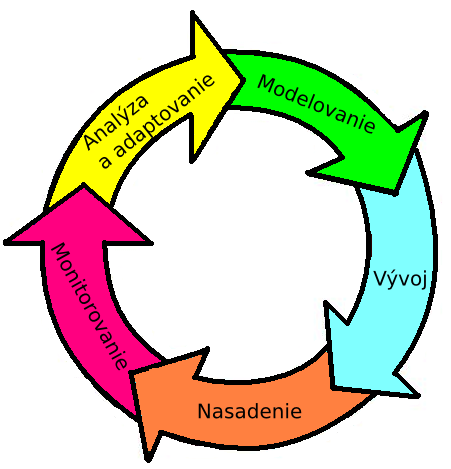
\includegraphics[width=300px]{pic/BDDmodel.png}
 \caption{Sch�ma �ivotn�ho cyklu navrhovanej met�dy.}
 \label{fig:mypic}
\end{figure}

\begin{description}
\item[Modelovanie firemn�ch procesov] -- ��elom  prvej f�ze v�vojov�ho procesu je za pomoci klienta zozbiera� po�iadavky na bud�ci syst�m. Sp�sa� �pecifik�ciu po�iadavkov a hlavne namodelova� firemn� procesy.  Po ods�hlasen� modelov z�kazn�kom sa ur�ia pr�pady u�itia a rozdel� sa funkcionalita. Z�kazn�k ur�� prioritu jednotliv�ch �alej vyv�jan�ch �ast�.
\item[N�vrh] -- Do n�vrhovej f�zy vstupuj� modely z predch�dzaj�cej �innosti. Tieto modely s�  spracovan� na n�vrh bud�ceho syst�mu. Pr�pady u�itia s� pop�san� pomocou krokov vypl�vaj�cich z krokov firemn�ch procesov. V pr�pade  potreby s� v zriedkav�ch pr�padoch bli��ie modelovan� sekven�n�mi diagramami. Statick� �trukt�ru budovan�ho syst�mu zachyt�vame pomocou diagramu tried. 

V�sledkom n�vrhovej �innosti je skromn� sada diagramov, ktor� musia by� kombinovan� s vopred vzniknut�mi diagramami firemn�ch procesov. Z�skan� v�sledn� sada modelov n�m dostato�ne popisuje bud�ci syst�m. Ako posledn� bod n�vrhovej �innosti je ur�en� architekt�ra, pomoci ktorej bude syst�m vyv�jan� (napr. Java, ASP .Net at�. ).
\item[V�voj] -- Pri implement�ci� bud�ceho syst�mu vych�dzame z vopred vypracovan�ch modelov a zvolenej architekt�ry. Rie�enie implementa�n�ch detailov na najni���ch �rovniach je ponechan� na odbornej znalosti program�tora. Probl�my s porozumen�m diagramov �i s k�dovan�m ur�itej �asti syst�mu je rie�en� komunik�ciou a dohodou v r�mci rie�ite�sk�ho t�mu. Kone�n�m produktom v�voja je testovate�n� �as� syst�mu.    
\item[Testovanie] -- Odha�ovanie ch�b je d�le�itou �as�ou ka�dej met�dy pou��vanej pri s��asnom v�voji  softv�ru. Z d�vodu zabezpe�enia maxim�lnej kvality ka�d�ho produktu nesmie by� t�to f�za opomenut� ani v navrhovanej met�de. Pri testovan� prejde syst�m sadou �tandardn�ch postupov testovania ako napr. automatizovan�mi testami, testami typu biela a �ierna skrinka, akcepta�n�mi testami at�. Pre nedostato�n�ch v�konnostn�ch v�sledkoch sa vykon�va rev�zia k�du. Softv�r, ktor� sp��a po�iadavky na funk�nos� a kvalitu je posunut� do �al�ej f�zy �ivotn�ho cyklu.        
\item[Nasadenie] -- Na z�ver je otestovan� �as� syst�mu nasaden� do prev�dzky.  Z�kazn�k m� mo�nos� pracova� s odovzdanou �as�ou syst�mu. V pr�pade vzniknutia neo�ak�van�ch nedostatkov produktu m��e z�kazn�k vy�iada� �pravu vyv�jan�ho rie�enia. Po �spe�nom nasaden� verzie syst�mu si m��e z�kazn�k ur�i� nasleduj�cu funkcionalitu, ktor� bude spracovan� a pridan� do produktu. V pr�pade nezmenia sa po�iadavkov pokra�uje cyklus pod�a vopred stanovenej priority v�voja �ast�.   
\end{description}  

\section{Vyu�it� role}
Procesy prebiehaj�ce v navrhnutej met�de vy�aduj� na zvl�dnutie znalosti z viacer�ch oborov informatiky a mana�mentu. Osoby pracuj�ce na v�voji softv�ru sa ocitaj� v nieko�k�ch preddefinovan�ch roliach. Ka�d� z rol� vykon�va �pecifick� �lohu po�as �ivotn�ho cyklu tvorenia produktu a je nepostr�date�n� na �spe�n� dosiahnutie cie�a. 

Preto�e sa venujeme produkovan�m mal�ch softv�rov�ch rie�en�, nie je pravdepodobn�, �e rie�ite�sk� t�m bude obsahova� ve�k� mno�stvo pracovn�kov. V�aka tomu, �e na produkovan� rie�enia sa bude podie�a� pomerne mal� t�m, umo�n� to intenz�vnu komunik�ciu a podporu medzi jeho �lenmi. Jednotliv� osoby sa po�as trvania projektu m��u dosta� do viacer�ch rol� v pr�pade, �e spl�uj� potrebn� kvalifik�ciu. 

Navrhovan� met�da definuje nasleduj�ce role:

\begin{description}
\item[Firemn� analytik] -- Jeho �lohou je komunikova� zo z�kazn�kom, pochopi� jeho potreby a fungovanie prostredia, do ktor�ho bude syst�m vyv�jan�. Na z�klade zozbieran�ch znalost� vypracuje firemn� analytik sadu modelov, ktor� zachytia procesy prebiehaj�ce v organiz�ci�. Opieraj�c sa o tieto diagramy komunikuje zo z�kazn�kom o jich korektnosti a spolo�ne s n�vrh�rom syst�mu m��u diskutova� o mo�n�ch vylep�eniach procesov.    
\item[N�vrh�r] -- Jeho hlavnou �lohou je zachytenie dynamickej a statickej �trukt�ry syst�mu. Vyu��va na to modely vyprodukovan� pri anal�ze podniku a komunikuje o rie�eniach s firemn�m analytikom. Vo firemn�ch procesoch identifikuje pr�pady u�itia, ��m zv�zuje tieto modely s modelmi, ktor� zachyt�vaj� n�vrh syst�mu. M� na starosti navrhnutie vykonate�n�ch technick�ch rie�en� k po�iadavk�m od z�kazn�ka. �lohou n�vrh�ra je tie� vo�ba vhodnej architekt�ry syst�mu po dohode so z�kazn�kom.  
\item[V�voj�r] -- M� na starosti prevedenie navrhnut�ch modelov do funguj�cej a nasadite�nej podoby. V��iu n�zko �rov�ov�ch ot�zok t�kaj�cich sa implementa�n�ch detailov m� na starosti vyrie�i� s�m. V pr�pade nepochopenia zadania alebo pri pr�padn�ch komplik�ci�ch pri svojej pr�ci m��e konzultova� ich rie�enia s n�vrh�rom.    
\item[Tester] -- M� na starosti overenie funkcionality a zaistenie kvality odovzdan�ho syst�mu. T�m �e pracuje s kone�nou funk�nou podobou �asti syst�mu, je t�to ro�a roz��ren� aj o zodpovednosti   t�kaj�ce sa nasadenia syst�mu. Pom�ha z�kazn�kovi po predan� produktu z jeho nasaden�m a poskytuje mu inform�cie t�kaj�ce sa jeho fungovania. Pr�padn� konfigurovanie produktu spad� tie� do povinnosti testera.        
\end{description}

Pre z�kazn�ka nie je stanoven� rola, lebo jeho poz�cia pri v�voji odpoved� jeho osobe. M� v�ak vo v�etk�ch prebiehaj�cich procesoch v�znamn� �lohu. Podie�a sa pri v�voji produktu a to nie len po�as po�iato�nej f�zy, ke� s� zbieran� po�iadavky na syst�m, ale akt�vne sa podie�a aj na ovplyv�ovan� vyv�jan�ho produktu po�as celej doby v�voja. Neseri�zny pr�stup k v�voju zo strany objedn�vate�a v�ne naru�uje �spe�nos� zvl�dnutia projektu a kvalitu odovzd�van�ho produktu.

\section{V�voj softv�rov�ho projektu}
V nasleduj�cej �asti tejto pr�ce sa budeme venova� postupu, ak�m bude softv�r vyv�jan� pomocou novo vyv�janej met�dy pre spracovanie mal�ch softv�rov�ch projektov. Pozornos� bude venovan� ka�dej f�zy �ivotn�ho cyklu a podrobne bud� pop�san� role a �innosti, ktor� sa jej z��ast�uj�. 

\subsection{�pecifik�cia po�iadavkov}
�vodn� �innos� pri vyv�jan� softv�rov�ho projektu mus� by� venovan� zbierania poznatkov o syst�me, ktor� budeme tvori�. T�to �innos� spad� do f�zy modelovania firemn�ch procesov. Firemn� analytik intenz�vne komunikuje zo z�kazn�kom. Pri vz�jomnej komunik�ci� si analytik objas�uje n�roky, ktor� bude z�kazn�k kl�s� na bud�ci syst�m. V pr�pade, �e s bud�cim syst�mom bude pracova� �ir�� okruch pracovn�kov vo firme, musia by� do zbierania po�iadavok zahrnut� aj oni. 

Na z�klade zozbieran�ch po�iadavkov od z�kazn�ka je zostaven� dokument �pecifik�cie po�iadaviek na bud�ci syst�m. Preto�e pracujeme z neve�k�mi projektami �pecifik�cia by nemala by� extr�mne rozsiahla a z�kazn�k by nemal ma� probl�m pre�tudova� ju a vyjadri� k nej svoje pripomienky. Po dokon�en� �pecifik�cie po�iadaviek a jej ods�hlasen� zo strany klienta m��eme post�pi� k �al�ej �innosti. \\

M�lnikom pre ukon�enie prvej �asti projektu je ods�hlasen� �pecifik�cia po�iadavkov. 

\subsection{N�vrh firemn�ch procesov}
Podobne ako predch�dzaj�ca �innos� spad� aj n�vrh firemn�ch procesov do  prvej f�zy �ivotn�ho cyklu. Sklad� sa z viacer�ch �innosti, ktor�ch cie�om je graficky spracova� dokument �pecifik�ci� po�iadaviek  z�skan� v predch�dzaj�cou �innos�ou. \\

Podrobn�m pre�tudovan�m �pecifik�cie a na z�klade z�skan�ch inform�ci� z prostredia, kde bude syst�m nasaden�, firemn� analytik za�ne modelova� firemn� procesy. Na ich modelovanie vyu��va BPMN. Vzniknut� modely podrobne popisuj� postup �innosti, ktor� ved� k vykonaniu ur�it�ho procesu vo firme. Jednotliv� diagramy obsahuj� okrem sledu �loh aj role zodpovedn� za vykonanie ur�it�ch �loh. V procesoch identifikujeme pas�e, ktor� m��u by� automatizovan� a pridel�me ich vykonanie syst�movej roli. Na pride�ovanie �innost� k roliam pou�ijeme koncepciu plaveck�ch dr�h, ktor� poskytuje BPMN. 

Odpor��an� sp�sob n�vrhu firemn�ch procesov je vyu�itie pr�stupu modelovania zhora na dol. Z�skavame t�m hierarchick� �trukt�ru diagramov, kde v najvy��ej �rovni zachyt�vame glob�lny poh�ad na hlavn� �innosti vykon�van� v organiz�ci�. Postupnou dekompoz�ciou t�chto hlavn�ch aktiv�t z�skavame podrobn� popis aktiv�t definovan�ch  na vy��ej �rovni. �lohy na najni��ej �rovni dekompoz�cie zachyt�vaj� atomick� �innosti, ktor� s� vo firme vykon�van�, a vyu��vaj� sa nesk�r ako kroky pr�padov u�itia. 

Po namodelovan� kompletnej hierarchie procesov, konzultujeme v�sledky zo z�kazn�kom a vykon�vame pr�padne nutn� �pravy. Po ods�hlasen� modelov zo strany z�kazn�ka nasleduje porada z n�vrh�rom syst�mu. Cel� syst�m je rozdelen� na men�ie �asti podla funkcionality, ktor� predstavuj� iter�cie. Vymedzen� oddiel mus� poskytova� ucelen� funkcionalitu, pr�nosn� pre z�kazn�ka. Jednotliv�m �astiam je priraden� priorita na z�klade klientov�ch po�iadavkov, podla ktorej je syst�m postupne vyv�jan�. Zostaven�m pl�nu ne ur�enie poradia iter�ci� a inkrementov je ukon�en� prv� f�za �ivotn�ho cyklu. \\

M�lnikmy pre f�zu n�vrhu firemn�ch procesov s� hierarchick� sada diagramov, ktor� popisuje bud�ci syst�m a pl�n iter�ci� a inkrementov pod�a ktor�ho bude syst�m postupne vyv�jan�. 

\subsection{Popis pr�padov u�itia}
Prvou �innos�ou n�vrhovej f�zy �ivotn�ho cyklu je spracovanie modelov firemn�ch procesov. Identifikujeme v nich pr�pady u�itia, ktor� graficky pop��eme �as�ami diagramov z ktor�ch sme vych�dzali.  



Previazanie BPMN a pr�padov u�itia
\subsection{Diagram tried}

\subsection{Vyvoj}

\subsection{Testovanie}

\subsection{Nasadenie a odovzdanie}

\chapter{Pr�padov� �t�dia}
\label{chap:appli}
Piata kapitola sa zaober� predveden�m navrhnutej met�dy z predch�dzaj�cej kapitoly. Overuje jej vhodnos� vytvoren�m pr�padovej �t�die popisuj�cej spr�vu vedeck�ho �asopisu. N�zorne s� predveden� �vodn� f�zy �ivotn�ho cyklu definovanej met�dy venovan� firemnej anal�ze a n�vrhu. Uk�ku implement�cie a n�sledn�ch �innost� u� t�to pr�ca nepon�ka.

�vod kapitoly je venovan� �pecifikovaniu po�iadavkov, ktor� tvoria z�klad pre modelovaciu f�zu. Popisuje sa tvorba hierarchie firemn�ch procesov pomocou BPMN a prechod od procesov k pr�padom pou�itia. N�zorne je predveden� ich previazanie s krokmi vo firemn�ch procesoch. V z�vere je e�te zachyten� statick� �trukt�ra syst�mu pomocou diagramu tried.

\section{�pecifik�cia po�iadavkov}
��elom syst�mu je zabezpe�enie vedeck�ho �asopisu. Webov� aplik�cia mus� ma� prvky redak�n�ho syst�mu, ktor� umo�nia administr�torovi upravova�, prid�va� a odobera� jej obsah. Aplik�cie bude zabezpe�ova� zbieranie a sprostredkov�vanie vedeck�ch �l�nkov. Na webovom rozhran� bud� zobrazovan� z�kladn� inform�cie o ka�dom �l�nku a to:
\begin{itemize}
\item autora 
\item in�tit�ciu
\item n�zov
\item k���ov� slov�
\item anot�ciu
\item odkaz na pln� text v PDF form�te pr�stupn� len pre registrovan�ch u��vate�ov
\end{itemize}
%Ku ka�d�mu �l�nku bude pripojen� diskusia, kde budu m�c� u��vatelia vyjadri� svoj n�zor k �l�nku a bud� ma� mo�nos� reagova� na koment�re in�ch u��vate�ov. Diskusia bude rozvrstven� podla logickej n�v�znosti koment�rov.

Aplik�cia bude obsahova� radu notifik�cii. Pri zalo�en� nov�ho ��tu bude zaslan� inform�cia administr�torovi so �iados�ou o jeho potvrdenie po overen� zaplatenia �lensk�ho poplatku. Pri ka�dom vlo�en� nov�ho �l�nku registrovan�m u��vate�om bud� vybran� a obozn�men� o tomto �l�nku recenzenti, ktor�ch �lohou bude �l�nok recenzova�. Registrovan� u��vatelia si m��u povoli� ozn�menie o nov�ch zverejnen�ch �l�nkoch cez e-mail. Po dov�en� limitu na zostavenie ��sla �asopisu bude o tom informovan� redak�n� rada a administr�tor. 

Inform�ci�ch ulo�en�ch v datab�ze bude mo�n� preh�ad�va�. Vyh�ad�vanie bude pod�a z�kladn�ch inform�cii okrem anot�cie. Taktie� sa nebude vyh�ad�va� v samotnom texte �l�nkov. Rozhranie vyh�ad�vania bude �o najjednoduch�ie. Bude poskytova� vo�by na ur�enie kateg�rie, v ktorej sa bude vyh�ad�va�:
\begin{itemize}
\item meno, in�tit�cia, n�zov
\item k���ov� slov�
\item ro�n�k 
\end{itemize}

\subsection{Konfigurovate�nos� a vzh�ad syst�mu}
Redak�n� prvky syst�mu umo�nia administr�torovi upravova� a dop��a� webov� rozhranie syst�mu. Bude ma� mo�nos� meni� logo port�lu, texty na str�nkach, prid�va� a zneplat�ova� nov� str�nky. V�etky zmeny rozlo�enia str�nok sa bud� prejavova� v �trukt�re menu str�nky, ktor� bude najviac dve �rov�ov�. Str�nky budu m�c� by� dopl�ovan� do ktorejko�vek �rovne menu. 

Webov� rozhranie bude umo��ova� zmenu vzh�adu pomocou dod�van�ch t�m. Aplik�cia bude vyhotoven� s jednou �tandardnou t�mou a s t�mou pre postihnut�ch. T�ma sa bude pre registrovan�ch u��vate�ov uklada� do ich profilu. 

Nevyhnutn� konfigur�cia hotovej distrib�cie prebehne pri jeho prvom spusten�. Vytvori sa tu administr�torsk� konto a v�etky nevyhnutn� nastavenia aplik�cie. Cel� nasleduj�ci beh syst�mu bude automaticky a v�etky pr�padne zmeny nastavenia a obsahu sa budu dia� cez webov� rozhranie administr�tora. Webov� rozhranie bude preh�adne, zamerane na r�chle dosiahnutie po�adovan�ch inform�ci�. Ka�d� str�nka mus� obsahova� tieto prvky:
\begin{itemize}
\item logo a z�kladne �daje o organiz�cii zria�uj�cej virtu�lnu konferenciu
\item menu str�nok webov�ho rozhrania
\item ak je u��vate� neprihl�sen� -- mo�nos� prihl�si� sa do syst�mu
\item ak je u��vate� prihl�sen� -- meno u��vate�a a vo�bu na odhl�senie sa
\end{itemize}
Inform�cie o ulo�en�ch �l�nkoch sa budu zobrazova� do preh�adn�ho v�pisu obsahuj�ceho z�kladn� inform�cie. Z�znamy sa bud� zobrazova� pre aktu�lny rok. Star�ie ro�n�ky bud� ulo�en� v arch�ve. Z�znamy pre aktu�lny ro�n�k budu chronologicky usporiadan� od najnov��ch po najstar�ie. Arch�v bude usporiadan� pod�a rokov a bude rovnako zoraden� ako aktu�lny ro�n�k. Parameter zora�ovanie bude m�c� u��vate� pozmeni� na meno, in�tit�ciu, n�zov a d�tum. Taktie� bude mo�nos� zmeni� vzostupnos� alebo zostupnos� usporiadania. V pr�pade, �e z�znamov bude viac ako limit zobrazenia na jednu str�nku, zoznam sa stane viac stranov�m. U��vate� si bude m�c� zvoli� ko�ko z�znamov chce na jedne kr�t zobrazi�.

\subsection{Definovan� role}
Aplik�cia bude rozli�ova� u��vate�ov, ktor� k nej budu pristupova�. Ka�d� u��vate�, ktor� sa neprihl�si bude ma� pr�vomoci neregistrovan�ho u��vate�a. Na registr�ciu bude k dispoz�cii formul�r na vytv�ranie nov�ch registorvan�ch u��vate�ov. Administr�torsk� ��et bude pridelen� u��vate�ovi pri inicializa�nom spusten� webovej aplik�cie. Pr�padn� �al�ie administr�torsk� ��ty mus� vytv�ra� u� existuj�ci administr�tor.
Syst�m rozozn�va nasledovne u��vate�sk� skupiny:
\begin{description}
 \item[Administr�tor] - Administr�tor bude ma� mo�nos� manipulova� s obsahom str�nok, spravova� u��vate�ov a m� na starosti prvotn� konfigur�ciu. V spr�ve u��vate�ov bude potvrdzova� nov� �iadosti o registr�ciu, bude m�c� pozme�ova� �daje o u��vate�ovi, meni� ich role a blokova� ��ty.
\item[Neregistrovan� u��vate�] - Bude ma� mo�nos� prehliada� zoznam ulo�en�ch �l�nkov, m��e v nich vyh�ad�va� ale nem� pr�stup k pln�m textom �l�nkov.
\item[\textbf{Registrovan� u��vate�}] - Bude ma� v�etky pr�va neregistrovan�ho u��vate�a a naviac aj pr�stup k pln�m textom �l�nkov z ro�n�ka, pre ktor� zaplatil �lensk� poplatok. Taktie� bude m�c� za z�kladn� �lensk� poplatok vlo�i� jeden �l�nok. Bude si m�c� upravova� inform�cie v profile a meni� pristupov� heslo.
\item[Redak�n� rada] - Bude ma� mo�nos� stopn�� uverejnenie pr�spevku s od�vodnen�m jeho pozastavenia.
\item[Recenzenti] - Bud� ma� pr�stup k textom �l�nkov v upravite�nej podobe a k odovzdan�m �l�nkom maj� mo�nos� prid�va� recenzovan� verziu.
\end{description}


\section{N�vrh firemn�ch procesov}
Modelovanie firemn�ch procesov za��na pre�tudovan�m �pecifik�cie po�iadavkov. Identifikuje sa v nej hlavn� proces, ktor� zachyt�me pomocou BPMN. Na u�ah�enie identifik�cie tohoto procesu pom��e ot�zka -- Ak�m hlavn�m �innostiam sa firma venuje? Vymedzen� �innosti graficky zachyt�me do diagramu pod�a ich postupnosti. 

\subsection{Identifik�cia hlavn�ho procesu}
Zo �pecifik�cie uvedenej v predch�dzaj�cej sekcii bol identifikovan� hlavn� proces tvoren� z piatich z�kladn�ch �ast�. Prv�m v l�nii vykonania je proces zabezpe�uj�ci autentiz�ciu u��vate�a a jeho autorizovanie. N�sledne proces pokra�uje podla pridelenej role. Neregistrovan� u��vate� si m��e prehliada� a vyh�ad�va� vo virtu�lnom �asopise alebo sa zaregistrova�. Registrovan� u��vate� m��e upravova� svoj profil a prida� �l�nok. Recenzenti pristupuj� k podprocesu recenzia �l�nku. Administr�tor m� na starosti spr�vu �asopisu. Redak�n� rada pristupuje k procesu zostavenia �asopisu. Po grafickom zachyten� postupnosti jednotliv�ch �innost� dost�vame prv� diagram syst�mu (\ref{fig:mainproc}) popisuj�ci syst�m na najvy��ej �rovni. 

\begin{figure}[ht]
 \centering
 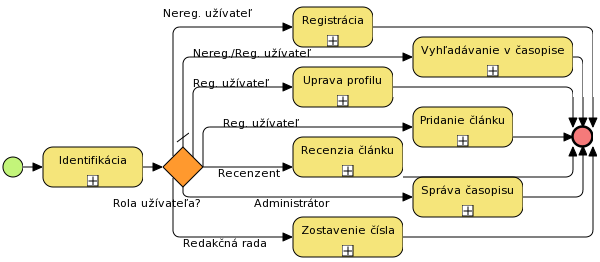
\includegraphics[width=350px]{pic/main.png}
  \caption{Diagram hlavn�ho firemn�ho procesu.}
 \label{fig:mainproc}
\end{figure}

Postupnou dekompoz�ciou hlavn�ho procesu je budovan� hierarchia modelov, ktor� popisuje funk�n� �trukt�ru organiz�cie a na najni��ej �rovni zachyt�va z�kladn� �innosti vykon�van� vo firme. Na nasleduj�com obr�zku \ref{fig:LL} je zachyten� postupn� dekompoz�cia jednej funk�nej �asti hlavn�ho procesu a� na najni��iu �rove�. Ke�e rozpracovanie celej hierarchie by bolo ve�mi pracn� a ako n�zorn� uk�ka posta�uje anal�za jednej vetvy, zvy�n� diagramy t�to prace obsahuje v dodatku A.

\begin{figure}[ht]
 \centering
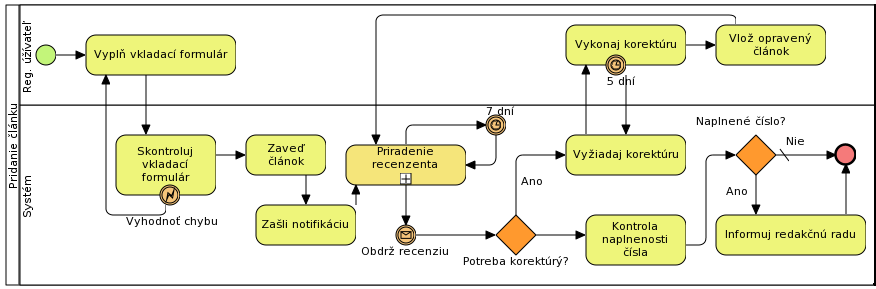
\includegraphics[width=\linewidth]{pic/pridaniec.png} 
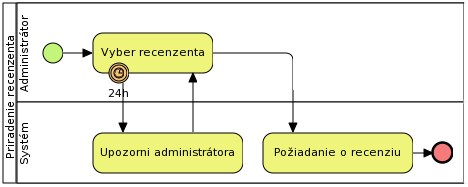
\includegraphics[width=250px]{pic/pridanierec.png}
  \caption{Dekompoz�cia pridania �l�nku.}
 \label{fig:LL}
\end{figure}

\subsection{Napl�novanie iter�cii a inkrementov}

Pomocou sch�my zachyt�vaj�cej hierarchick� �trukt�ru procesov prebiehaj�cich vo firme je mo�n� pokra�ova� v �al�om pl�novan�. Funkcionalita cel�ho syst�mu je rozdelen� na �asti  definovan� pre �ah�ie zvl�dnutie projektu a r�chlej�ie poskytnutie funkcionality z�kazn�kovo. Obr�zok \ref{fig:hs} zachyt�va rozdelenie syst�mu virtu�lneho �asopisu. 

\begin{figure}[ht]
 \centering
 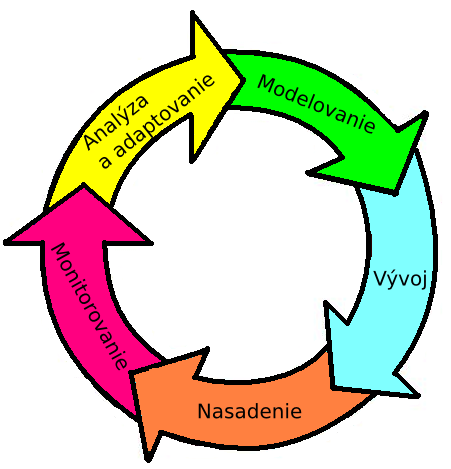
\includegraphics[width=100px]{pic/BDDmodel.png}
  \caption{Sch�ma hierarchickej �trukt�ry procesov.}
 \label{fig:hs}
\end{figure}

Po identifik�cii funk�n�ch �ast� je rozdelenie prediskutovan� so z�kazn�kom. Objedn�vate� na z�klade svojich najnutnej��ch potrieb ur�� poradie dod�van�ch komponent. Pre uk�kov� projekt je za prim�rnu �ast syst�mu ozna�en� funkcionalita poskytuj�ca jednoduch� prelistovanie a vkladania �l�nkov do virtu�lneho �asopisu. K z�kladnej funkcionalite patria aj u��vate�sk� role. U��vatelia sa bud� m�c� registrova� prihlasova�, meni� svoje �daje a pr�stup ku pln�m zneniam �l�nkov bude obmedzen� len pre registrovan�ch u��vate�ov. Po zvl�dnut� identifik�cie u��vate�a je spracovan� �as� syst�mu umo��uj�ca recenzovanie a zostavovanie ��sla �asopisu. N�sledne je syst�m roz��ren� o mo�nos� vyh�ad�vanie v datab�ze �l�nkov a upravovanie profilu u��vate�a. Ako posledn� funkcionalita je spr�stupnen� spr�va syst�mu pre administr�tor. Umo��uje mu �pravu obsahu webov�ho rozhrania.

\subsection*{Nasleduj�ci zoznam zora�uje iter�cie podla postupnosti poradia v�voja:}

\begin{enumerate}
\item Jednoduch� zobrazenie, vkladanie �l�nkov a u��vate�sk� role
\item  Recenzovanie a zostavovanie ��sla �asopisu
\item  Vyh�ad�vanie a �prava profilu
\item  Spr�va syst�mu
\end{enumerate}

\section{N�vrh syst�mu}

Pomocou diagramov vypracovan�ch v predch�dzaj�cej f�ze prist�pime k n�vrhu syst�mu. Pod�a pl�nu iter�cii budeme postupne vypracov�va� jednotliv� �asti syst�mu. Ako prv� funkcionalita, ktor� m� by� vyprodukovan� je vkladanie �l�nkov a ich jednoduch� zobrazenie. 

\subsection{Prv� iter�cia}
Zoberieme si diagramy firemn�ch procesov popisuj�ce procesy spojen� s vkladan�m �l�nku (obr. \ref{fig:hs}). S� na �om vidite�n� s�visl� automatizovate�n� �asti vykon�van� syst�mom, ktor� poskytuj� dobr�ch kandid�tov na pr�pady pou�itia. Z diagramu taktie� m��eme vy��ta� akt�rov. Jasne vidite�n� akt�ri s� \textit{registrovan� u��vate�} a \textit{administr�tor} posledn� trochu skryt�m je \textit{�as}. Po malej �vahe zist�me, �e okrem pr�padov pou�itia pre vlo�enie knihy, vy�iadanie recenzie a korekt�ry je vhodne vymedzi� aj pr�pad u�itia zabezpe�uj�ci notifik�ciu. 

Zavedenie rol do syst�mu vy�aduje funkcionalitu na ich vytvorenie a overenie. Obr�zoky \ref{fig:vytrol} a \ref{fig:overrol} zobrazuj� diagramy zachyt�vaj�ce �lohy spojen� s vytvoren�m a overen�m registrovan�ho u��vate�a. Pribudol v nich nov� akt�r a to \textit{u��vate�}. Pr�pady pou�itia pozorovate�n� v modeloch sa t�kaj� vytvorenia registr�cie s vy�iadan�m �hrady poplatku a jej potvrdenie. Z druh�ho firemn�ho procesu identifikujeme pr�pad pou�itia pre prihl�senie sa. 

\begin{figure}[ht]
 \centering
  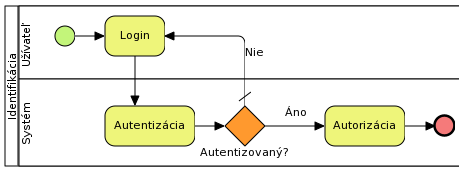
\includegraphics[width=240px]{pic/login.png}
  \caption{Proces overenie u��vate�a.}
 \label{fig:overrol}
\end{figure}

\begin{figure}[ht]
 \centering
 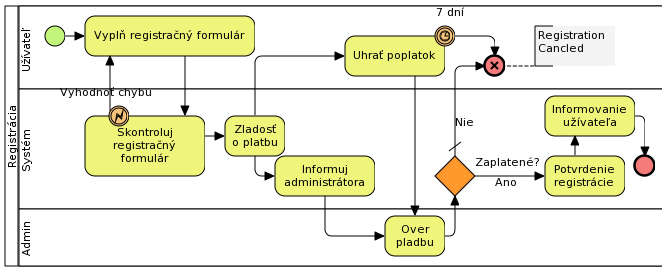
\includegraphics[width=400px]{pic/registracia.png}
   \caption{Diagramy popisuj�ce vytvorenie u��vate�a.}
 \label{fig:vytrol}
\end{figure}

\subsection*{Pr�pady pou�itia}
\begin{figure}[ht]
 \centering
 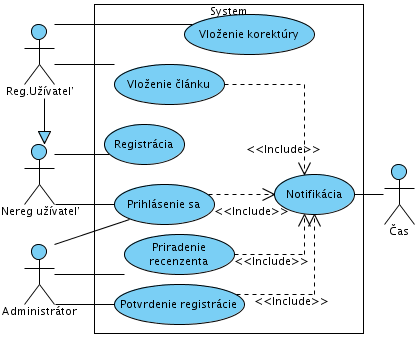
\includegraphics[width=320px]{pic/UC1.png}
  \caption{Diagram pr�padov pou�itia prvej iter�cie.}
 \label{fig:uc1}
\end{figure}

\begin{description}
\item[Vlo�enie �l�nku] -- Sklad� sa z troch krokov ur�en�ch v diagrame firemn�ch procesov. Prv�m je kontrola zad�van�ch �dajov pri vkladan� �l�nku, nasleduje jeho nahranie. Na z�ver je  vyu��va \textit{notifik�ciu} na zaslanie inform�cie o pridan� �l�nku.
\item[Priradenie recenzenta] -- Za��na v�berom recenzenta, ktor� je skrz \textit{notifik�ciu} informovan� o potrebnej recenzii. Recenzentovi bude zaslan� informa�n� e-mail s odkazom na �l�nok k ohodnoteniu. Formul�r pre zav�dzanie recenzii bude pridan� a� v druhej  iter�cii, preto je do�asne zasielanie recenzie rie�en� priamou cestou bez vyu�itia syst�mu.
\item[Vlo�enie korekt�ry] --  Autor m� mo�nos� po prihl�sen� sa vlo�i� opravu �l�nku do syst�mu, po ktorom je op� spusten� \textit{priradenie recenzenta}.
\item[Notifik�cia] -- Upozor�uje dan�ch u��vate�ov o v�skyte udalosti. Zaslanie m��e by� vyn�ten� alebo pravidelne prebieha rozosielanie �asovo podmienen�ch spr�v. Vyu��va na to e-mail zadan� pri registr�cii.
\item[Prihl�senie sa] -- Od u��vate�a je vy�iadan� meno a heslo, ktor� je s vyu�it�m he�ovania a dat ulo�en�ch v datab�ze overen�.
\item[Registr�cia] -- U��vate� po vyplnen� formul�ru obdr�� variabiln� symbol a ��slo ��tu pre uhradenie �lensk�ho poplatku administr�tor je pomocou \textit{notifik�cie} informovan� o novej registr�cii.
\item[Potvrdenie registr�cie] -- Administr�tor po overen� platby aktivuje ��et uch�dza�ovi o registr�ciu a je mu zaslan� e-mail o schv�len� registr�cie. 
\end{description}


\subsection*{Statick� �trukt�ra}
Diagram tried (obr.: \ref{fig:dt1}) zachyt�vaj�ci statick� �trukt�ru syst�mu budujeme za pomoci vypracovan�ho modelu pr�padov pou�itia. Na �vod s� na�rtnut� hrub� obrysy diagramu, ktor� je postupne spres�ovan�. Za v�stup iter�cie sa pova�uje presn� n�vrhov� diagram tried zachyten� na obr�zku \ref{fig:uc1}.

Diagram obsahuje ... .



\begin{figure}[ht]
 \centering
 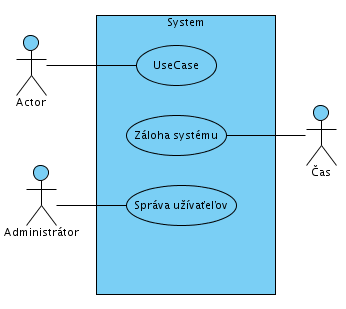
\includegraphics[width=200px]{pic/usecaseex.png}
  \caption{Diagram pr�padov pou�itia prvej iter�cie.}
 \label{fig:dt1}
\end{figure}

\subsection{Druh� iter�cia}

Po dokon�en� pr�ci na prvej iter�cii a posunutie ich v�sledkov do f�zy v�voja za��na pre n�vrh�ra pr�ca na �al�ej iter�cii. Druh� iter�cia ma za cie� roz��ri� doteraz vytvoren� syst�m o �as� pre recenzovanie �l�nkov a umo�ni� redak�nej rade zostavi� ��slo �asopisu. Zober� sa preto firemn� procesy popisuj�ce tieto �innosti (obr.: \ref{fig:recacas}). Taktie� je potrebn� doplni� spracovanie recenzie pop�san� na diagrame \ref{fig:LL}.

Z diagramov popisuj�cich procesy m��eme identifikova� dvoch akt�rov. S recenziami je spojen� textit{recenzent}  hodnotiaci �l�nok a vytv�raj�ci recenziu. Druh�m akt�rom je \textit{redak�n� rada} maj�ca na starosti zostavovanie ��sla �asopisu, ke� je dosiahnut� limit potrebn� na jeho naplnenie. \textit{Redak�n� rada} m� pr�vo na vyl��enie �l�nku. 

\begin{figure}[ht]
 \centering
 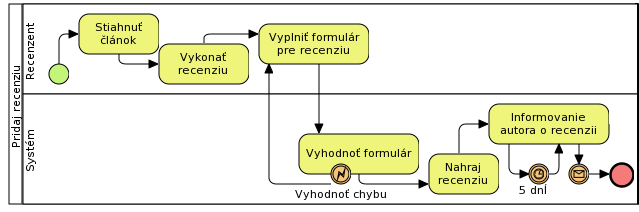
\includegraphics[width=400px]{pic/pridajrecenziu.png}
 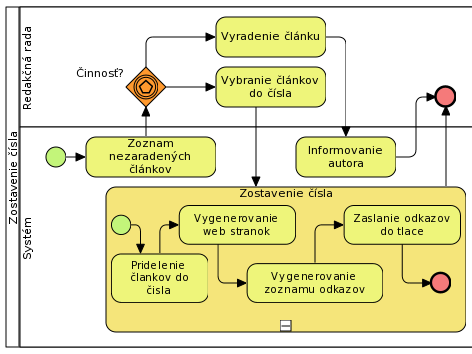
\includegraphics[width=260px]{pic/zostaveniecis.png}
  \caption{Model recenzovania a zostavovania ��sla �asopisu.}
 \label{fig:recacas}
\end{figure}


\subsection*{Pr�pady pou�itia}
\begin{description}
\item[Vlo�enie recenzie] -- Recenzent po vypracovan� hodnotenia vst�pi do syst�mu a vypln� formul�r pre recenziu. Syst�m formul�r skontroluje a ak je v�etko v poriadku recenzia je nahran� a autor je pomocou \textit{notifik�cie} informovan� o vykonanej recenzii. Recenzent uv�dza pri zad�van� recenzie �i je potrebn� korekt�ra. V pr�pade, �e je korekt�ra potrebn� je autor informovan� o tomto fakte. Ak korekt�ra nie je zapotreby je u� len skontrolovan� stav naplnenia �asopisu. Ak bolo odovzdan�ch dostatok �l�nkov je informovan� redak�n� rada.
\item[Zostavenie ��sla] -- Pri zostaven� ��sla je redak�nej rade zobrazen� zoznam doru�en�ch publik�cii. Rada si v zozname ozna�� �l�nky, ktor� zarad� do bud�ceho ��sla a taktie� m��e �l�nky podla zv�enia zo zoznamu vyl��i�. Autorom vyl��en�ch �l�nkov bud� o tom informovan�. Po ur�en� obsahu vydania s� �l�nky zaradene do ��sla v DB, pre ��slo je vygenerovan� vlastn� webov� str�nka. Je zostaven� zoznam odkazov na pln� texty �l�nkov a tento zoznam je zaslan� do tla�e.  
\item[Notifik�cia] -- Na upozor�uje u��vate�ov o v�skyte udalosti sa vyu��va notifik�cia navrhnut� v prvej iter�cii.
\end{description}

\begin{figure}[ht]
 \centering
 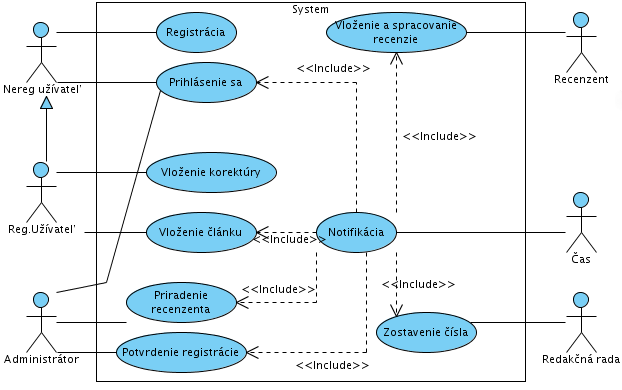
\includegraphics[width=400px]{pic/UC2.png}
  \caption{Diagram pr�padov pou�itia po druhej iter�cii.}
 \label{fig:uc2}
\end{figure}

\subsection*{Statick� �trukt�ra}

V druhej iter�cii bol diagram tried roz��ren� o treidy ... .

\begin{figure}[ht]
 \centering
 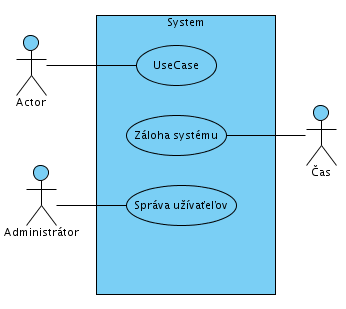
\includegraphics[width=200px]{pic/usecaseex.png}
  \caption{Diagram pr�padov pou�itia prvej iter�cie.}
 \label{fig:CD2}
\end{figure}

\subsection{Z�ver n�vrhu}
\chapter{Z�ver}
\label{chap:zaver}
V s��asnej dobe je v�voj softv�ru u� takmer nepredstavite�n� bez vyu�itia nejakej modelovacej met�dy, ktor� tento v�voj dok�e usmerni�, napom�c� z�skanie kvalitn�ho rie�enia probl�mu a rap�dne zv��i� �spe�nos� projektu. R�zne met�dy maj� rozdielne �pecifick� prvky a niektor� je potrebn� prisp�sobi� adekv�tnemu vyu�itiu a maximalizovaniu potenci�lu skr�vaj�ceho sa v nich. V�berom a pr�padnou �pravou postupu modelovania je zv��en� efekt�vnos� pr�ce, ur�chlen� v�voja a zn��en� n�klady na projekt. D�sledkom je dod�vanie kvalitn�ho softv�ru v dostupn�ch cenov�ch rel�ci�ch.

V�eobecne je hlavnou my�lienkou pou��vania metod�k u�ah�enie zvl�dnutia ve�k�ch projektov. Ke� v�ak aplikujeme rozsiahle a robustn� met�dy na mal�, jednoducho pochopite�n� a zvl�dnute�n� projekty, z�skavame zna�n� po�et �innost� nepos�vaj�cich projekt k r�chlemu koncu. Ve�k� po�et definovan�ch rol a modelov, ktor� musia by� vypracovan�, spoma�uje prechod k vlastn�mu produkovaniu syst�mu. Tento pr�stup ur�ite pon�ka monument�lny z�klad pre v�voj aplik�ci�, ale pre z�kazn�ka nemus� dod�va� rie�enia dostato�ne r�chlo. Pr�ve z�kazn�k potrebuje r�chle zavedenie IT rie�enia, aby zostala zachovan� jeho konkurencieschopnos�. Pri zd�havom dod�van� produktu m��e nasta� situ�cia, �e syst�m nesp��a r�chlo sa meniace po�iadavky klienta.

Na�tudovanie rozli�n�ch modelovac�ch met�d vyu��van�ch v minulosti a s��asnosti sl��ilo ako z�klad pre n�vrh met�dy umo��uj�cej efekt�vny v�voj mal�ch softv�rov�ch projektov. Popri pre�tudovan� modelov bolo cie�om tejto pr�ce aj obozn�menie sa s grafick�mi modelovac�mi n�strojmi, hlavne s Business Process Modeling Notation, sl��iacim na popisovanie firemn�ch procesov.

Navrhnut� met�da vyu��va BPMN diagramy na zachytenie po�iadaviek u��vate�a ako jeden zo vstupov do analytickej a v�vojovej �asti. Tieto diagramy s� intuit�vne pre z�kazn�ka, ktor� na z�klade nich m��e s analytikom diskutova� o dodanej funkcionalite realizovan�ho syst�mu. V�pr�pade, �e cie�ov� organiz�cia u� m� pop�san� �trukt�ru fungovania pomocou procesov, je t�m v�voj v�razne ur�chlen�.

Hlavn�m cie�om met�dy je r�chle dod�vanie kvalitn�ch IT rie�en� plniacich aktu�lne z�kazn�kove potreby. V navrhnutom postupe sa preto uplat�uj� my�lienky zachyten� v manifeste agiln�ho programovania. Vyzdvihovan� je spolupr�ca so z�kazn�kom a upravovanie n�vrhu a v�voja pod�a jeho predst�v. 

BPMN diagramy zachyt�vaj� funkcionalitu bud�ceho syst�mu. Charakterom pou�itia maj� prvky diagramov d�tov�ch tokov, ktor� boli v minulosti pou��van� pri n�vrhu softv�ru. Z�skava sa tak pomerne intuit�vny n�h�ad na fungovanie syst�mu, ktor� ke� spoj�me s diagramami tried pou��van�mi pri objektovo orientovanom n�vrhu, d�vaj� program�torovi jasn� rys budovan�ho syst�mu, ale tie� mu ponech�vaj� dostato�n� priestor na zapojenie svojej kreativity do realizovania v�sledn�ho rie�enia.

Navrhnut� met�da bola overen� pri vypracovan� informa�n�ho syst�mu pre spr�vu vedeck�ho �asopisu. Pod�a stanoven�ho postupu boli zachyten� po�iadavky na syst�m, ktor� boli preveden� na BPMN modely, a s ich pomocou boli vypracovan� diagramy pr�padov pou�itia a tried. Postupn� odvodzovanie diagramov prebehlo bez v���ch probl�mov. Z�skan� v�sledn� s�bor modelov popisuje statick� a dynamick� �trukt�ru produktu. 

Na �pln� overenie met�dy v�ak ch�ba realiz�cia navrhnut�ch modelov, ktor� v�ak nem��e by� preveden� tou istou osobou ako n�vrhov� �as�. Je potrebn� n�h�ad druhej, nezainteresovanej osoby, ktor� nem� so syst�mom sk�senosti a musela by sa preto spolieha� len na poskytnut� modely a komunik�ciu s n�vrh�rom. Overila by sa t�m miera zrozumite�nosti a mno�stvo inform�ci� poskytovan�ch modelmi.

\bibliographystyle{plain}  % bibliografick� styl 
\begin{thebibliography}{6}
\bibitem{BPMNINT}
White, Stephen A. \textit{Introduction to BPMN} [online].[cit. 2009-3-2].
Dostupn� na internete: $<$http://www.omg.org/spec/BPMN/1.2/PDF$>$

\bibitem{BPMNSPEC}
Object Management Group. \textit{Business Process Modeling Notation (BPMN)} [online]. Jan 2009 [cit. 2009-3-2].
Dostupn� na internete: $<$http://www.bpmn.org/Documents/Introduction\%20to\%20BPMN.pdf$>$

\bibitem{AGIL}
 Keith, Everette R. \textit{Agile Software Development Processes: A Different Approach to Software Design} [online]. 1. Dec 2002 [cit. 2009-4-16].
Dostupn� na internete: $<$http://www.agilealliance.com/system/article/file/1099/file.pdf$>$

\bibitem{BDD}
Mitra, T. \textit{Business-driven development} [online]. Dec 2005 [cit. 2009-3-2].
Dostupn� na internete: $<$http://www.ibm.com/developerworks/webservices/library/ws-bdd/$>$
\end{thebibliography}



\appendix 
\chapter{Pr�loha A}
%fsafas
\end{document}